\documentclass[12pt,a4paper,oneside]{report}
\usepackage[margin=1in,headheight=16pt]{geometry}
\usepackage[T1]{fontenc}
\usepackage[utf8]{inputenc}
\usepackage{lmodern,microtype,graphicx,booktabs,tabularx,longtable,array,adjustbox}
\usepackage{amsmath,amssymb,siunitx,algorithm,algpseudocode}
\usepackage{xcolor,tikz,caption,subcaption,float,fancyhdr,tocloft,titlesec,enumitem}
\usepackage{etoolbox}
\usepackage[unicode,hidelinks]{hyperref}
\usepackage[nameinlink,noabbrev]{cleveref}
\usetikzlibrary{arrows.meta,positioning,fit,calc,shapes.geometric}
\definecolor{Forest}{HTML}{152C24}
\definecolor{Leaf}{HTML}{147D55}
\definecolor{Soft}{HTML}{EDF3EE}
\definecolor{CollegeBlue}{HTML}{174E82}
\definecolor{TitleRed}{HTML}{B8343E}
\definecolor{Muted}{HTML}{58665F}
\linespread{1.15}
\setlength{\parskip}{3pt}
\setlength{\parindent}{0pt}
\setlength{\emergencystretch}{2em}
\renewcommand{\topfraction}{.95}
\renewcommand{\bottomfraction}{.95}
\renewcommand{\textfraction}{.05}
\renewcommand{\floatpagefraction}{.8}
\setcounter{totalnumber}{5}
\setcounter{topnumber}{5}
\setcounter{bottomnumber}{3}
\setlength{\floatsep}{12pt plus 2pt minus 2pt}
\setlength{\textfloatsep}{12pt plus 2pt minus 2pt}
\setlength{\intextsep}{12pt plus 2pt minus 2pt}
\setlist{nosep,leftmargin=*}
\captionsetup{font=small,labelfont=bf,skip=8pt}
\titleformat{\chapter}[display]{\normalfont\color{Forest}\bfseries}{\large CHAPTER \thechapter}{7pt}{\LARGE}
\titlespacing*{\chapter}{0pt}{-12pt}{18pt}
\titleformat{\section}{\large\bfseries\color{Forest}}{\thesection}{.7em}{}
\titleformat{\subsection}{\normalsize\bfseries\color{Forest}}{\thesubsection}{.7em}{}
\titlespacing*{\section}{0pt}{11pt}{5pt}
\titlespacing*{\subsection}{0pt}{8pt}{4pt}
\setcounter{tocdepth}{0}
\renewcommand{\bibname}{References}
\pagestyle{fancy}
\fancyhf{}
\fancyhead[L]{\small\nouppercase{\leftmark}}
\fancyhead[R]{\small 23DS7BSBIO}
\fancyfoot[L]{\small Department of CSE (Data Science)}
\fancyfoot[R]{\thepage}
\renewcommand{\headrulewidth}{.3pt}
\renewcommand{\footrulewidth}{.3pt}
\fancypagestyle{plain}{\fancyhf{}\fancyhead[R]{\small 23DS7BSBIO}\fancyfoot[L]{\small Department of CSE (Data Science)}\fancyfoot[R]{\thepage}\renewcommand{\headrulewidth}{0pt}\renewcommand{\footrulewidth}{.3pt}}
\graphicspath{{../figures/}{../assets/}}
\newcommand{\ProjectTitle}{Plant Disease Detection using Transfer-Learning CNN Optimized with Differential Evolution}
\newcommand{\RepoURL}{https://github.com/Suraj-B12/BIO-INSPIRED-ALGO---AAT}
\newcommand{\PageBorder}{\begin{tikzpicture}[remember picture,overlay]\draw[Forest!60,line width=.8pt,rounded corners=10pt] ($(current page.north west)+(15mm,-15mm)$) rectangle ($(current page.south east)+(-15mm,15mm)$);\end{tikzpicture}}
\newcommand{\PendingResult}{\textit{Pending final evaluation}}
\IfFileExists{generated/numbers.tex}{% Generated by scripts/10_make_tables.py; never edit result numbers by hand.
\newcommand{\ResultsComplete}{1}
\newcommand{\BaseAcc}{97.43}
\newcommand{\BaseAccStd}{0.45}
\newcommand{\BasePrecision}{96.73}
\newcommand{\BasePrecisionStd}{0.61}
\newcommand{\BaseRecall}{96.53}
\newcommand{\BaseRecallStd}{0.48}
\newcommand{\BaseFone}{96.60}
\newcommand{\BaseFoneStd}{0.54}
\newcommand{\BaseAUC}{99.94}
\newcommand{\BaseAUCStd}{0.02}
\newcommand{\BaseStd}{0.45}
\newcommand{\BaseAccCI}{[97.13, 98.24]\%}
\newcommand{\BaseFoneCI}{[96.15, 97.70]\%}
\newcommand{\BaseECE}{0.81}
\newcommand{\BaseRobustAcc}{85.77}
\newcommand{\BaseParams}{330506}
\newcommand{\DEAcc}{99.85}
\newcommand{\DEAccStd}{0.06}
\newcommand{\DEPrecision}{99.82}
\newcommand{\DEPrecisionStd}{0.10}
\newcommand{\DERecall}{99.79}
\newcommand{\DERecallStd}{0.10}
\newcommand{\DEFone}{99.80}
\newcommand{\DEFoneStd}{0.09}
\newcommand{\DEAUC}{100.00}
\newcommand{\DEAUCStd}{0.00}
\newcommand{\DEStd}{0.06}
\newcommand{\DEAccCI}{[99.63, 99.96]\%}
\newcommand{\DEFoneCI}{[99.48, 99.95]\%}
\newcommand{\DEECE}{9.23}
\newcommand{\DERobustAcc}{69.19}
\newcommand{\DEParams}{4338054}
\newcommand{\RSAcc}{99.85}
\newcommand{\RSAccStd}{0.04}
\newcommand{\RSPrecision}{99.80}
\newcommand{\RSPrecisionStd}{0.05}
\newcommand{\RSRecall}{99.81}
\newcommand{\RSRecallStd}{0.07}
\newcommand{\RSFone}{99.80}
\newcommand{\RSFoneStd}{0.06}
\newcommand{\RSAUC}{100.00}
\newcommand{\RSAUCStd}{0.00}
\newcommand{\RSStd}{0.04}
\newcommand{\RSAccCI}{[99.74, 100.00]\%}
\newcommand{\RSFoneCI}{[99.69, 100.00]\%}
\newcommand{\RSECE}{8.85}
\newcommand{\RSRobustAcc}{Pending}
\newcommand{\RSParams}{4649460}
\newcommand{\BaselineParams}{330,506}
\newcommand{\McNemarP}{\num{9.048e-15}}
\newcommand{\ErrorReduction}{94.29}
\newcommand{\BestLR}{\num{0.001257}}
\newcommand{\NumEvals}{72}
\newcommand{\TotalN}{18,146}
\newcommand{\DataOriginal}{18,160}
\newcommand{\DataDuplicates}{14}
\newcommand{\DataCorrupt}{0}
\newcommand{\TrainN}{12,701}
\newcommand{\ValN}{2,723}
\newcommand{\TestN}{2,722}
\newcommand{\BenchmarkRuns}{30}
\newcommand{\BenchmarkBudget}{20,000}
\newcommand{\TotalBenchmarkRuns}{750}
\newcommand{\TotalBenchmarkEvaluations}{15,000,000}
\newcommand{\BenchmarkSeconds}{105.34}
\newcommand{\SphereDE}{\num{2.59e-15}}
\newcommand{\DeviceName}{mps}
\newcommand{\CPUName}{Apple M4 Pro}
\newcommand{\TorchVersion}{2.15.0}
\newcommand{\PythonVersion}{3.11.14}
\newcommand{\MemoryGB}{48}
\newcommand{\ComputeTier}{B}
\newcommand{\RepoCommit}{5e28dddf8220}
\newcommand{\RepoRevisionSource}{Project Git HEAD}
\newcommand{\FinalEpochs}{15}
\newcommand{\BatchSize}{32}
\newcommand{\Resolution}{224}
\newcommand{\SeedCount}{3}
}{}
\providecommand{\ResultsComplete}{0}
\providecommand{\BaseAcc}{Pending}\providecommand{\DEAcc}{Pending}\providecommand{\RSAcc}{Pending}
\providecommand{\BaseFone}{Pending}\providecommand{\DEFone}{Pending}\providecommand{\RSFone}{Pending}
\providecommand{\DEStd}{Pending}\providecommand{\McNemarP}{Pending}\providecommand{\ErrorReduction}{Pending}
\providecommand{\BestLR}{Pending}\providecommand{\NumEvals}{Pending}
\providecommand{\TrainN}{Pending}\providecommand{\ValN}{Pending}\providecommand{\TestN}{Pending}\providecommand{\TotalN}{Pending}
\providecommand{\DataOriginal}{Pending}\providecommand{\DataDuplicates}{Pending}\providecommand{\DataCorrupt}{Pending}
\providecommand{\BenchmarkRuns}{Pending}\providecommand{\BenchmarkBudget}{Pending}\providecommand{\SphereDE}{Pending}
\providecommand{\TotalBenchmarkRuns}{Pending}\providecommand{\TotalBenchmarkEvaluations}{Pending}\providecommand{\BenchmarkSeconds}{Pending}
\providecommand{\DeviceName}{Pending}\providecommand{\ComputeTier}{Pending}\providecommand{\CPUName}{Pending}\providecommand{\MemoryGB}{Pending}
\providecommand{\TorchVersion}{Pending}\providecommand{\PythonVersion}{Pending}\providecommand{\RepoCommit}{Pending}
\providecommand{\RepoRevisionSource}{Unavailable}
\providecommand{\BaselineParams}{Pending}\providecommand{\DEParams}{Pending}
\providecommand{\BaseFoneCI}{Pending}\providecommand{\DEFoneCI}{Pending}\providecommand{\BaseAccCI}{Pending}\providecommand{\DEAccCI}{Pending}
\providecommand{\BaseECE}{Pending}\providecommand{\DEECE}{Pending}\providecommand{\BaseRobustAcc}{Pending}\providecommand{\DERobustAcc}{Pending}
% Short list-of-figures entries keep the front matter compact.
\newcommand{\ArtifactFigureShort}[5][.95]{%
  \IfFileExists{../figures/#2.pdf}{\begin{figure}[htbp]\centering\includegraphics[width=#1\linewidth,height=.64\textheight,keepaspectratio]{#2.pdf}\caption[#3]{#4}\label{#5}\end{figure}}{%
  \IfFileExists{../figures/#2.png}{\begin{figure}[htbp]\centering\includegraphics[width=#1\linewidth,height=.64\textheight,keepaspectratio]{#2.png}\caption[#3]{#4}\label{#5}\end{figure}}{\begin{quote}\small\textcolor{Muted}{Figure awaiting its measured source artifacts: \texttt{\detokenize{#2}}.}\end{quote}}}}
\newcommand{\ArtifactFigure}[4][.95]{\ArtifactFigureShort[#1]{#2}{#3}{#3}{#4}}
% Two complementary plots share one float, each with its own numbered caption.
\newcommand{\ArtifactFigurePair}[8]{%
  \IfFileExists{../figures/#1.pdf}{\IfFileExists{../figures/#5.pdf}{%
    \begin{figure}[htbp]\centering
    \includegraphics[width=\linewidth,height=.42\textheight,keepaspectratio]{#1.pdf}
    \caption[#2]{#3}\label{#4}\par\vspace{10pt}
    \includegraphics[width=\linewidth,height=.42\textheight,keepaspectratio]{#5.pdf}
    \caption[#6]{#7}\label{#8}
    \end{figure}}{\ArtifactFigureShort[1]{#1}{#2}{#3}{#4}\ArtifactFigureShort[1]{#5}{#6}{#7}{#8}}}{%
    \ArtifactFigureShort[1]{#1}{#2}{#3}{#4}\ArtifactFigureShort[1]{#5}{#6}{#7}{#8}}}
\newcommand{\ArtifactTable}[3]{\begin{table}[htbp]\centering\caption{#2}\label{#3}\small\IfFileExists{generated/#1.tex}{\begin{adjustbox}{max width=\textwidth}\input{generated/#1.tex}\end{adjustbox}}{\PendingResult}\end{table}}
\hypersetup{pdftitle={\ProjectTitle},pdfauthor={Team 10, B.M.S. College of Engineering},pdfsubject={Bio-Inspired Algorithms, 23DS7BSBIO}}
\patchcmd{\thebibliography}{\chapter*{\bibname}}{\chapter{\bibname}}{}{}
\begin{document}
\hypersetup{pageanchor=false}
\begin{titlepage}
\PageBorder
\centering
{\Large\bfseries\color{CollegeBlue} B.M.S. COLLEGE OF ENGINEERING\par}
\vspace{3pt}
{\small (Autonomous College under VTU)\par}
{\small Bull Temple Road, Basavangudi, Bangalore - 560019\par}
\vspace{10pt}

\includegraphics[height=25mm]{bmsce_logo.png}\par
\vspace{8pt}
{\large Bio Inspired Algorithms AAT on\par}
{\small Course Code: \textbf{23DS7BSBIO}\par}
\vspace{8pt}
{\Large\bfseries\color{TitleRed}\ProjectTitle\par}
\vspace{12pt}
{\small in fulfillment of the requirements for the award of degree\par}
{\normalsize\bfseries BACHELOR OF ENGINEERING\par}
{\small in\par}
{\normalsize\bfseries Computer Science \& Engineering (Data Science)\par}
\vspace{10pt}
{\small by\par}
\vspace{5pt}
\begin{tabular}{ll}
\textbf{Aryanraj S Singh} & \textbf{1BM23CD008}\\
\textbf{Richik Chaudhuri} & \textbf{1BM23CD050}\\
\textbf{Suraj B} & \textbf{1BM23CD061}\\
\textbf{Sushant Deo} & \textbf{1BM23CD062}
\end{tabular}
\vspace{14pt}

{\small Under the Guidance of\par}
{\normalsize\bfseries Manoj Kumar S\par}
{\small Assistant Professor\par}
{\small Department of CSE (Data Science), B.M.S. College of Engineering\par}
\vfill
{\normalsize\bfseries AY 2026--2027\par}
{\small Team 10\par}
\end{titlepage}
\pagenumbering{roman}
\hypersetup{pageanchor=true}
\thispagestyle{empty}\PageBorder
\begin{center}
{\Large\bfseries\color{CollegeBlue} B.M.S. COLLEGE OF ENGINEERING}\par
{\small (Autonomous College under VTU)}\par
{\small Department of Computer Science \& Engineering (Data Science)}\par
\vspace{5pt}
\includegraphics[height=19mm]{bmsce_logo.png}\par
\vspace{5pt}{\Large\bfseries CERTIFICATE}\par
\end{center}
\small
This is to certify that the project entitled ``\ProjectTitle'' is a bona fide work carried out by the following students for the course Bio Inspired Algorithms (Course Code: \textbf{23DS7BSBIO}). It is certified that all corrections and suggestions indicated during the internal assessments have been incorporated in the final report submitted to the departmental library. The project report has been approved as it meets the academic requirements prescribed for the Bachelor of Engineering Degree in respect of project work.\par
\vspace{8pt}
\renewcommand{\arraystretch}{1.55}
\begin{tabularx}{\textwidth}{@{}c l l X@{}}
\toprule
Sl. No. & Student Name & USN & Student's Signature\\\midrule
1 & Aryanraj S Singh & 1BM23CD008 & \\
2 & Richik Chaudhuri & 1BM23CD050 & \\
3 & Suraj B & 1BM23CD061 & \\
4 & Sushant Deo & 1BM23CD062 & \\\bottomrule
\end{tabularx}\par
\renewcommand{\arraystretch}{1}
\vspace{25pt}
\begin{minipage}[t]{.46\textwidth}
Signature of the Guide\par
\vspace{17pt}\textbf{Manoj Kumar S}\par
Assistant Professor
\end{minipage}\hfill
\begin{minipage}[t]{.46\textwidth}
Signature of the HOD\par
\vspace{17pt}\textbf{Dr. Shyamala G}\par
Professor \& HOD
\end{minipage}
\vspace{25pt}

\textbf{Examiners}\par
\vspace{5pt}
\begin{tabularx}{\textwidth}{@{}c X X@{}}
\toprule & Name of Examiner & Signature\\\midrule
1 & & \\[12pt]
2 & & \\[12pt]\bottomrule
\end{tabularx}
\begin{center}Academic Year 2026--2027\end{center}
\normalsize\clearpage
\chapter*{Acknowledgement}
\addcontentsline{toc}{chapter}{Acknowledgement}
We thank the Principal of B.M.S. College of Engineering and the management of B.M.S. Educational Trust (BMSET) for providing the academic environment and facilities for this work.

We express our gratitude to \textbf{Dr. Shyamala G, Professor \& Head of the Department, Computer Science and Engineering (Data Science)}, for departmental support. We thank our guide \textbf{Manoj Kumar S, Assistant Professor}, for guidance in the Bio-Inspired Algorithms course and for encouraging clear connections between algorithm design, implementation, and experimental evidence.

We also thank the department faculty, the maintainers of the open-source scientific software used in this project, and the researchers who made PlantVillage and the cited research openly accessible. Their contributions make transparent and reproducible student research possible.

The team takes responsibility for the implementation, the integrity of the reported experimental evidence, and the limitations stated in this report. No signature is reproduced electronically; the certificate provides spaces for the required academic sign-off.

\vspace{18pt}
\begin{flushright}
Aryanraj S Singh\par
Richik Chaudhuri\par
Suraj B\par
Sushant Deo\par
\textbf{Team 10}
\end{flushright}
\clearpage
\chapter*{Abstract}
\addcontentsline{toc}{chapter}{Abstract}
This project evaluates Differential Evolution (DE) for selecting an ImageNet-pretrained EfficientNet-B0 training recipe for tomato disease classification. The backbone, dataset, baseline, and evaluation protocol are fixed before selection. A normalized chromosome controls learning rate, weight decay, dropout, classifier width, fine-tuning depth, label smoothing, and augmentation. DE/rand/1/bin is implemented from scratch with distinct donors, parent-to-bound repair, forced crossover, greedy selection, and resumable state.

The cleaned dataset contains \TotalN\ images, partitioned into \TrainN\ training, \ValN\ validation, and \TestN\ test images using visual-similarity groups. Validation macro-F1 guides proxy search and higher-fidelity reranking. Selected recipes undergo repeated final training; random search supplies an equal-budget control. Evaluation covers per-class performance, bootstrap intervals, paired correctness, calibration, corruptions, and Grad-CAM. Analytic benchmarks separately assess optimizer behavior.

\ifnum\ResultsComplete=1\relax
Mean accuracy is \BaseAcc\% for the baseline and \DEAcc\% for both searched recipes; DE and random search tie in mean accuracy. Baseline, DE, and random-search macro-F1 scores are \BaseFone\%, \DEFone\%, and \RSFone\%, respectively. However, DE's mean corruption accuracy is lower than the baseline's (\DERobustAcc\% versus \BaseRobustAcc\%), and its seed-zero calibration error is higher (\DEECE\% versus \BaseECE\%). Improved clean classification therefore does not establish better field reliability or superiority over random search.
\else
The current build reports completed data preparation and optimizer benchmarks; final neural-network results remain explicitly pending. No anticipated accuracy is substituted for a measured result.
\fi

An offline demo connects predictions and optimizer evolution to saved evidence. The contribution is a reproducible comparison with explicit trade-offs, rather than a universally superior classifier.
\clearpage

\tableofcontents
\clearpage\listoffigures
\clearpage\listoftables
\clearpage\pagenumbering{arabic}
\chapter{Introduction}
\section{Background and problem}
Crop pathogens and pests impose substantial losses, with effects that vary by crop and geography~\cite{savary2019losses}. Official Indian horticulture statistics establish tomato as a substantial production crop~\cite{pib2026tomato}. Leaf imagery therefore offers a useful application for accessible visual screening. PlantVillage studies demonstrate classification on curated images~\cite{hughes2015dataset,mohanty2016plant}; they also motivate careful separation of benchmark performance from field reliability.

This project asks whether Differential Evolution (DE) can improve an ImageNet-pretrained EfficientNet-B0 tomato classifier by selecting its training recipe. The objective is validation macro-F1 over a mixed space of learning rate, regularization, head width, fine-tuning depth, and augmentation. Backpropagation fits each candidate's weights; DE selects the recipe. The dataset, backbone family, and optimizer topic remain fixed.

\section{Measurable objectives}
\begin{enumerate}
\item Prepare documented class mappings, cleaning records, and group-aware stratified splits.
\item Implement and test DE donor selection, mutation, repair, crossover, and selection.
\item Compare a registered baseline, DE, and equal-budget random search using validation-only selection.
\item Evaluate repeated seeds, per-class performance, uncertainty, robustness, and calibration.
\item Deliver an offline demonstration and reproducible report, slides, code, and evidence.
\end{enumerate}

\section{Contribution, scope, and organization}
The contribution is an auditable chain from candidate vector to checkpoint and reported result. Established methods are combined and evaluated; no claim of a new optimizer or universal superiority is made. Curated-dataset accuracy does not establish reliability for arbitrary crops, unknown diseases, or field photographs.

Chapters 2--4 develop the literature and algorithms; Chapters 5--6 specify implementation and evaluation. Chapters 7--8 analyze the evidence. Applications, conclusions, future work, verified references, and repository instructions complete the report.

\chapter{Literature Review}
\section{Image-based plant disease classification}
Hughes and Salathé released the PlantVillage collection of labelled plant-leaf photos to support research on automatic diagnosis~\cite{hughes2015dataset}. Mohanty et al. trained deep networks on it and reached very high accuracy, while noting that photos taken in real fields are harder~\cite{mohanty2016plant}. Ferentinos tested several CNN designs on a larger multi-crop collection~\cite{ferentinos2018plant}. Too et al. compared fine-tuned networks and found DenseNet performed best~\cite{too2019plant}. Each of these studies uses its own classes and data splits, so their numbers are not directly comparable with ours.

Kamilaris and Prenafeta-Boldú review the wider use of deep learning in agriculture~\cite{kamilaris2018survey}. PlantDoc collects leaf photos taken outside the laboratory~\cite{singh2020plantdoc}, and Gui et al. study how background and lighting in field photos affect recognition~\cite{gui2021field}. These works show that field photos are an important next step after laboratory datasets.

\section{Transfer learning and efficient networks}
EfficientNet grows a network in a balanced way by scaling its depth, width, and input image size together~\cite{tan2019efficientnet}. We use its smallest version, B0, and tune how it is trained. MobileNetV2 and MobileNetV3 are other compact networks designed for phones~\cite{sandler2018mobilenet,howard2019mobilenet}.

Yosinski et al. show that early layers of a trained network learn general features, while later layers become specific to the original task~\cite{yosinski2014transfer}. This means the number of layers we retrain (the fine-tuning depth) is an important choice. Keeping the whole pretrained network fixed is a simple, common baseline. Retraining more layers can adapt better to leaves, but costs more time. We let the search decide.

\section{Hyperparameter and evolutionary search}
Grid search tries every combination from a fixed list of values; random search simply tries randomly chosen settings. Bayesian optimisation builds a model of which settings are likely to work well~\cite{snoek2012bayesian}. Hyperband saves time by stopping weak trials early~\cite{li2016hyperband}. Random search is a strong and simple competitor, so we use it as our control: it tells us whether DE's guided search adds value over picking the same number of settings at random.

Evolutionary methods have been used successfully to design and tune networks. Real et al. used an evolutionary method to design image classifiers~\cite{real2019evolution}. Wang et al. used particle swarm optimisation and a hybrid DE method to design CNNs~\cite{wang2018psoarchitecture,wang2018dearchitecture}. DEHB combines DE with Hyperband for tuning~\cite{awad2021dehb}. These results motivate applying DE to our seven training settings.

\begin{table}[htbp]\centering\small
\caption{Published results, each measured on its own dataset and protocol.}
\begin{tabularx}{\textwidth}{@{}>{\raggedright\arraybackslash}p{.19\textwidth}>{\raggedright\arraybackslash}X >{\raggedright\arraybackslash}p{.23\textwidth}r@{}}\toprule
Study & Dataset / model & Search or comparison & Accuracy\\\midrule
Mohanty et al.~\cite{mohanty2016plant} & PlantVillage, 38 classes; AlexNet/GoogLeNet & Training/model variants & 99.35\%\\
Ferentinos~\cite{ferentinos2018plant} & 58 categories; CNNs & CNN architectures & 99.53\%\\
Too et al.~\cite{too2019plant} & PlantVillage, 38 classes; DenseNet & Fine-tuned architectures & 99.75\%\\
Gui et al.~\cite{gui2021field} & Field-PV; adapted CNN & Background/features & 72.03\%\\\bottomrule
\end{tabularx}
\end{table}

\section{Research gap}
Most earlier plant-disease studies choose training settings by hand. Few apply an evolutionary search to these settings and compare it fairly with a fixed baseline and with random search at the same cost. This project fills that gap for tomato leaves: it uses fair data splits, a baseline fixed in advance, the same number of trials for each search method, and repeated final training runs. It also links the algorithm to a working offline demo.

\chapter{Theoretical Background}
\section{CNNs and transfer learning}
A CNN slides small learned filters over an image to detect local patterns such as edges and spots. Stacking many such layers lets the network recognise larger shapes and textures. EfficientNet-B0 is built from efficient blocks called MBConv, which include a small ``attention'' step (squeeze-and-excitation) that tells the network which feature channels matter most. EfficientNet scales depth $d$, width $w$, and image resolution $r$ together as $d=\alpha^\phi$, $w=\beta^\phi$, $r=\gamma^\phi$ with $\alpha\beta^2\gamma^2\approx2$~\cite{tan2019efficientnet}. We keep the B0 size.

On top of the network we place a small \emph{classifier head}: dropout, an optional hidden layer, and ten outputs, one per class. The softmax function $p_c=\exp(z_c)/\sum_j\exp(z_j)$ turns the ten outputs $z_c$ into probabilities that add up to one. Layers that are ``frozen'' keep their pretrained values; ``unfrozen'' layers are retrained on tomato leaves. Retraining later layers helps because they hold the most task-specific features~\cite{yosinski2014transfer}.

\section{Training and regularisation}
Training minimises the cross-entropy loss $\mathcal L=-N^{-1}\sum_i\sum_c q_{ic}\log p_{ic}$, which is small when the model gives high probability to the correct class. Several settings help the model generalise instead of memorising:
\begin{itemize}
\item \textbf{Dropout} randomly switches off some connections during training.
\item \textbf{Weight decay} keeps the network's weights small.
\item \textbf{Label smoothing} softens the target answers slightly, $q_{ic}=(1-\epsilon)y_{ic}+\epsilon/C$, so the model is less over-confident.
\item \textbf{Augmentation} shows randomly flipped, cropped, and colour-changed versions of each image.
\end{itemize}
The baseline uses the Adam optimiser; the searched recipes use AdamW, a version of Adam with built-in weight decay. The learning rate rises briefly at the start (warm-up) and then decreases smoothly (cosine schedule). Training stops early when validation macro-F1 stops improving, and the best checkpoint is kept.

\section{Classification metrics}
For class $c$, $TP_c$ counts correct detections, $FP_c$ false alarms, and $FN_c$ missed cases:
\begin{align}
P_c&=\frac{TP_c}{TP_c+FP_c}, & R_c&=\frac{TP_c}{TP_c+FN_c}, & F_{1,c}&=\frac{2P_cR_c}{P_c+R_c},\\
F_{1,\mathrm{macro}}&=\frac{1}{C}\sum_cF_{1,c}, & \mathrm{Accuracy}&=\frac{1}{N}\sum_i\mathbf1[\hat y_i=y_i].
\end{align}
Precision $P_c$ asks ``when the model says class $c$, how often is it right?''; recall $R_c$ asks ``how many real class-$c$ leaves did it find?''; F1 balances the two. Macro-F1 averages F1 over all classes, so every disease counts equally. The ROC curve shows how well the model separates one class from the rest at every confidence threshold, and its area (AUC) is 100\% for perfect separation.

\section{Statistical checks}
\emph{Bootstrap confidence intervals} give a plausible range for a score by repeatedly re-sampling the test images~\cite{efron1979bootstrap}. The \emph{McNemar test} compares two models on the same test images. It looks only at the images where exactly one model is right and checks whether this split could happen by chance~\cite{dietterich1998tests}. A very small $p$-value means the difference is real.

\section{Calibration, explanations, and robustness}
A model is well \emph{calibrated} when its confidence matches how often it is right. Expected calibration error (ECE) measures the gap, averaged over confidence bins $B_m$~\cite{guo2017calibration}:
\begin{equation}
\mathrm{ECE}=\sum_{m=1}^{M}\frac{|B_m|}{N}\left|\mathrm{acc}(B_m)-\mathrm{conf}(B_m)\right|.
\end{equation}
\emph{Grad-CAM} produces a heat map showing which parts of the image most influenced the prediction~\cite{selvaraju2017gradcam}. \emph{Corruption tests} add blur, noise, or darkness to test images to see how the model copes with poorer photos~\cite{hendrycks2019corruptions}.

\chapter{Nature-Inspired Algorithms: Detailed Study}
\section{Classification and shared search principles}
Metaheuristics guide search without a useful analytic optimum. Population methods maintain several candidates; trajectory methods modify one state. Exploration visits new regions, while exploitation refines promising ones.

\begin{figure}[htbp]\centering
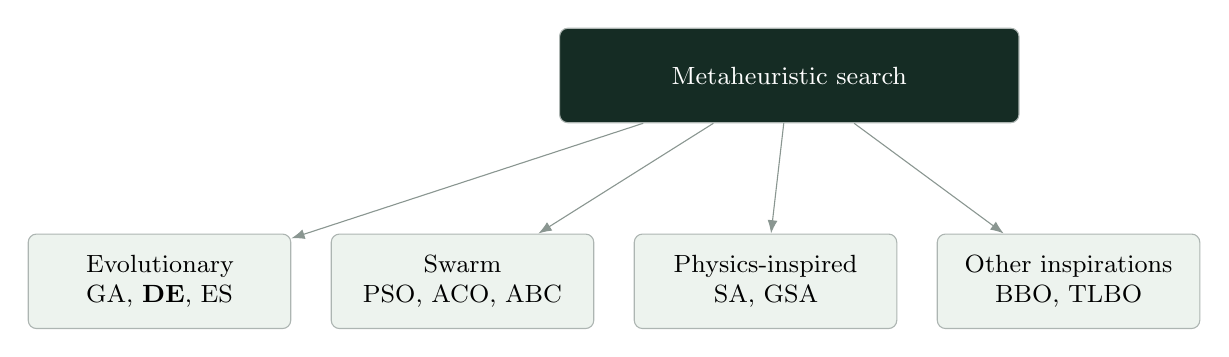
\begin{tikzpicture}[node distance=7mm,box/.style={draw=Forest!35,rounded corners=3pt,fill=Soft,align=center,text width=31mm,minimum height=12mm,font=\small},arr/.style={-{Latex},Forest!50}]
\node[box,text width=56mm,fill=Forest,text=white] (root) {Metaheuristic search};
\node[box,below left=14mm and 34mm of root] (e) {Evolutionary\\GA, \textbf{DE}, ES};
\node[box,right=5mm of e] (s) {Swarm\\PSO, ACO, ABC};
\node[box,right=5mm of s] (p) {Physics-inspired\\SA, GSA};
\node[box,right=5mm of p] (o) {Other inspirations\\BBO, TLBO};
\draw[arr] (root)--(e);\draw[arr] (root)--(s);\draw[arr] (root)--(p);\draw[arr] (root)--(o);
\end{tikzpicture}
\caption{A teaching taxonomy. BBO is biogeography-inspired; categories overlap and do not rank algorithm quality.}
\end{figure}

GA combines selection and variation~\cite{holland1992adaptation}; PSO maintains individual and social memories~\cite{kennedy1995pso}. Ant System uses pheromone feedback~\cite{dorigo1996aco}; simulated annealing uses temperature-controlled acceptance~\cite{kirkpatrick1983annealing}.

\section{Representative update mechanisms}
A real-coded GA recombines selected parents, for example $\mathbf u=\alpha\mathbf x_a+(1-\alpha)\mathbf x_b$, then mutates and selects survivors. Our comparator uses tournament selection, blend crossover, Gaussian mutation, and elitism.

For PSO, particle velocity and position are updated as
\begin{align}
\mathbf v_i^{t+1}&=w\mathbf v_i^t+c_1\mathbf r_1\odot(\mathbf p_i-\mathbf x_i^t)+c_2\mathbf r_2\odot(\mathbf g-\mathbf x_i^t),\\
\mathbf x_i^{t+1}&=\mathbf x_i^t+\mathbf v_i^{t+1},
\end{align}
where $\mathbf p_i$ is the particle's best position and $\mathbf g$ the population best. In an ant system, transition preference is proportional to pheromone $\tau_{ij}^{\alpha}$ times heuristic desirability $\eta_{ij}^{\beta}$; pheromone is evaporated and reinforced by completed solutions~\cite{dorigo1996aco}. Simulated annealing accepts an uphill energy change $\Delta E$ with probability $\exp(-\Delta E/T)$, allowing controlled escape from local basins~\cite{kirkpatrick1983annealing}.

Firefly-style movement combines attraction and random perturbation, often expressed as $\mathbf x_i\leftarrow\mathbf x_i+\beta_0e^{-\gamma r_{ij}^2}(\mathbf x_j-\mathbf x_i)+\alpha\boldsymbol\epsilon$~\cite{yang2009firefly}. BBO models immigration and emigration between candidate habitats; a simple linear rate model uses $\lambda(s)=I(1-s/S)$ and $\mu(s)=Es/S$ for species count $s$~\cite{simon2008bbo}. ABC uses employed/onlooker/scout search roles~\cite{karaboga2007abc}; GWO models social hierarchy and hunting-inspired position updates~\cite{mirjalili2014gwo}. These are background methods, not additional CNN experiments.

\section{Differential Evolution in depth}
DE maintains $NP$ vectors in a normalized domain. In DE/rand/1, mutation for target $i$ is
\begin{equation}
\mathbf v_i=\mathbf x_{r_1}+F(\mathbf x_{r_2}-\mathbf x_{r_3}),\qquad r_1,r_2,r_3\ne i,
\end{equation}
with distinct donor indices. Difference vectors supply directions and scales informed by the current population~\cite{storn1997de,das2011survey}. The implementation freezes the donor population within each generation, so earlier evaluations do not change later donors in the same generation.

For a coordinate outside $[0,1]$, the repair rule draws a feasible value between the parent and the violated bound:
\begin{equation}
v_{ij}\leftarrow x_{ij}+r(b-x_{ij}),\quad r\sim U(0,1),\quad b\in\{0,1\}.
\end{equation}
Valid coordinates remain unchanged. This repair avoids repeated clipped boundary values but does not preserve uniform sampling.

Binomial crossover forms
\begin{equation}
u_{ij}=\begin{cases}v_{ij},&r_j<CR\ \text{or}\ j=j_{\mathrm{rand}},\\x_{ij},&\text{otherwise}.\end{cases}
\end{equation}
The forced coordinate ensures mutant contribution. Maximizing selection is
\begin{equation}
\mathbf x_i^{g+1}=\begin{cases}\mathbf u_i,&f(\mathbf u_i)\ge f(\mathbf x_i^g),\\\mathbf x_i^g,&\text{otherwise}.\end{cases}
\end{equation}
Best stored fitness is nondecreasing, although noisy fitness can misrepresent true quality. Difference-vector mutation is rotation-equivariant; coordinate-wise crossover prevents the whole algorithm from being rotation-invariant.

\begin{figure}[H]\centering
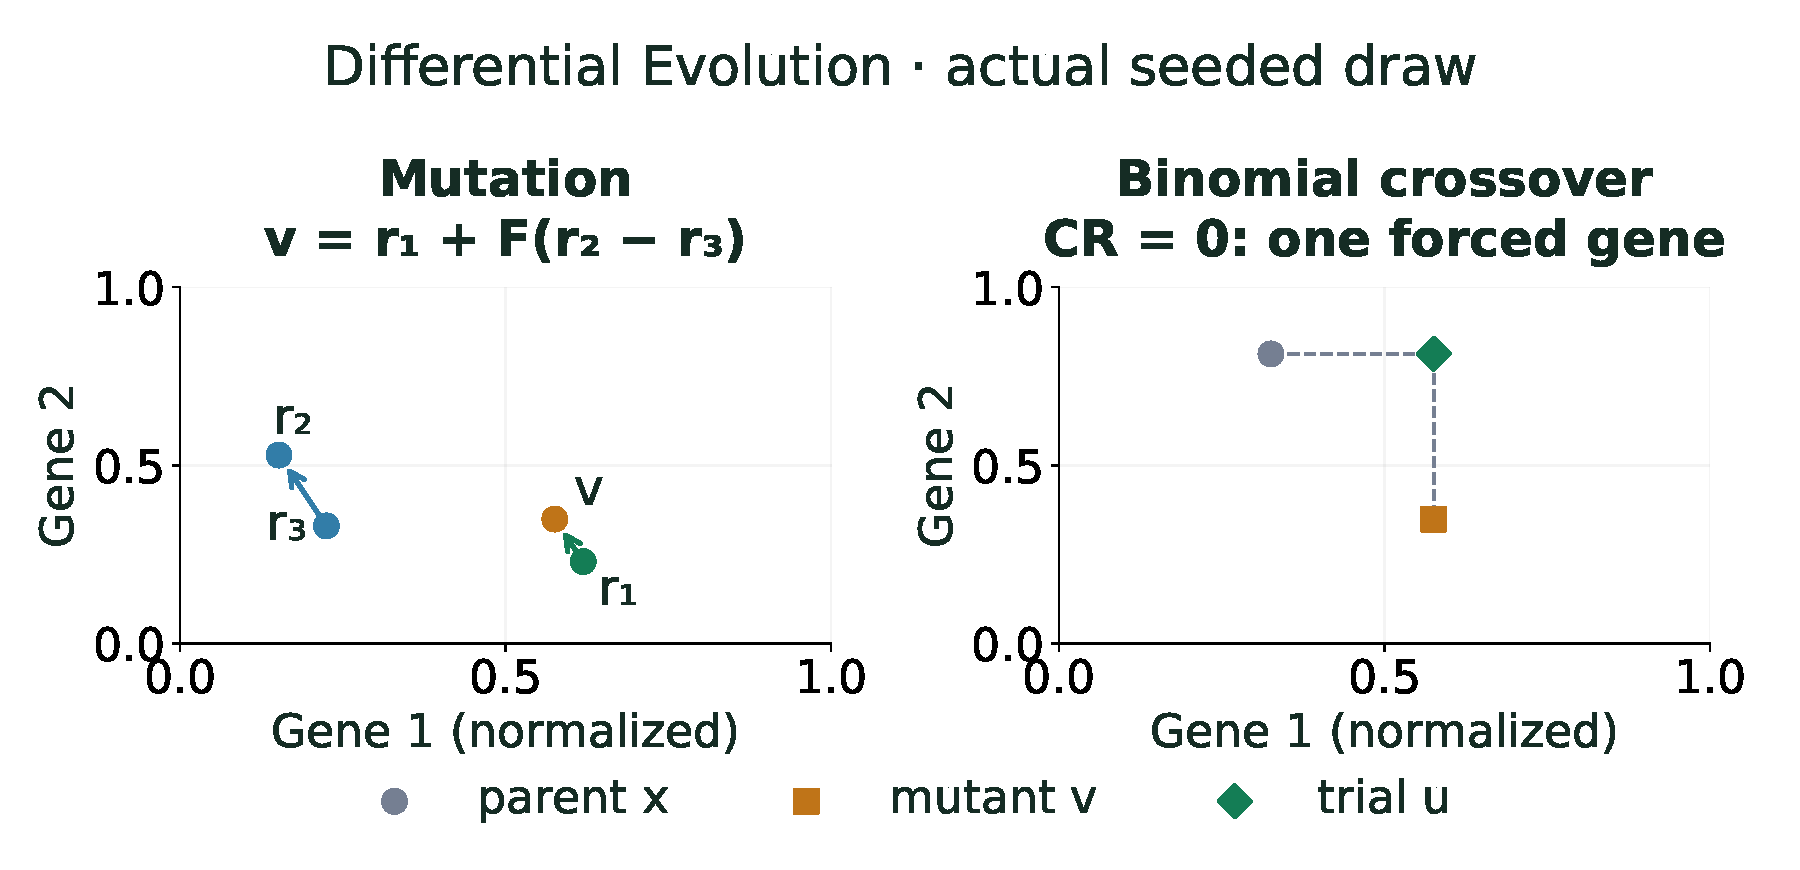
\includegraphics[width=.75\linewidth]{fig_de_operators_diagram.pdf}
\caption{Mutation, bound repair, and crossover using a recorded operator example.}\label{fig:deoperators}
\end{figure}

\section{Pseudocode and complexity}
\begin{algorithm}[H]
\caption{DE/rand/1/bin with deferred generation donors}
\begin{algorithmic}[1]
\Require Objective $f$, dimension $D$, population $NP$, generations $G$, $F$, $CR$
\State Initialize $X$ with Latin-hypercube samples in $[0,1]^D$
\State Evaluate all initial candidates and persist state
\For{$g=1,\ldots,G$}
\State $S\gets X$ \Comment{Frozen donor population}
\For{$i=1,\ldots,NP$}
\State Choose three distinct donor indices excluding $i$
\State $v\gets S_{r_1}+F(S_{r_2}-S_{r_3})$
\State Repair violating coordinates between $X_i$ and the bound
\State Form $u$ using binomial crossover and forced $j_{\mathrm{rand}}$
\State Evaluate $f(u)$ using the same fitness protocol
\If{$f(u)\ge f(X_i)$}\State $X_i\gets u$\EndIf
\State Atomically persist population, scores, and RNG state
\EndFor
\State Record fitness distribution, diversity, and success rate
\EndFor
\State \Return best recorded vector and full history
\end{algorithmic}
\end{algorithm}

The budget is $NP(G+1)$ including initialization; vector arithmetic is $O(GNP D)$, while training dominates time. Mean pairwise distance measures diversity, and replacement fraction measures success rate; both help identify stagnation.

\section{Variants and parameter control}
DE/best/1 uses the current best as its mutation base; DE/rand/2 uses two difference vectors; current-to-best strategies add attraction toward a leading vector. Such changes modify exploration and exploitation~\cite{das2016recent}. Increasing $F$ expands differential steps, while $CR$ changes coordinate mixing; their useful values depend on the landscape and available budget.

jDE retains successful individual control values~\cite{brest2006jde}; SHADE uses success histories and L-SHADE reduces population size~\cite{tanabe2013shade,tanabe2014lshade}. Only classic DE optimizes this CNN; adaptive variants are benchmark comparators.

\textbf{Why DE here.} Seven normalized genes support derivative-free mixed search with few controls and independent candidate evaluations. Noisy fitness, repeated recipes, and small populations limit coverage; equal-budget evidence determines usefulness~\cite{sorensen2015metaphors}.

\chapter{Methodology and Implementation}
\section{Overall pipeline}
The work runs in four stages: prepare the data, search for the best settings, retrain the chosen recipes, and test them once on held-out images. Each stage is a numbered Python script, and a few small shared modules hold the data, model, training, and optimiser code. The offline demo uses the saved results and trained models.

\ArtifactFigureShort{fig_pipeline}{System pipeline}{The project pipeline, from data preparation to search, final evaluation, and the offline demo.}{fig:pipeline}

\section{Data preparation and splitting}
We downloaded the colour tomato images from the public PlantVillage repository. The ten class folders, sorted alphabetically, define the class labels. Every image was checked to open correctly and converted to standard RGB colour. Exact duplicate images were removed. Images that look almost identical (for example, two photos of the same leaf) were grouped together and always placed in the same split, so the model is never tested on a near-copy of a training image.

The raw data had \DataOriginal\ images. We removed \DataDuplicates\ duplicates and found \DataCorrupt\ broken files, leaving \TotalN\ images. These were split about 70/15/15 into training, validation, and test sets, keeping the class proportions the same in each split. The split lists are saved in the repository so every run uses exactly the same images.

\ArtifactTable{tab_data_summary}{Number of images per class and split after cleaning.}{tab:data}

\section{Image preparation}
Images are resized once and cached to make training faster. During training, each image is randomly cropped and flipped; the searched recipes can also add RandAugment, which applies random colour and shape changes of a chosen strength. The baseline uses only cropping and flipping. Validation and test images are simply resized and centre-cropped, with no randomness.

\section{Model and baseline}
We use EfficientNet-B0 with ImageNet weights and the classifier head from Chapter~3. The network body has nine blocks. The \emph{fine-tuning depth} $k$ says how many of the last blocks are retrained: $k=0$ trains only the head, and $k=9$ retrains the whole network. The baseline trains \BaselineParams\ parameters.

\ArtifactFigureShort{fig_architecture}{EfficientNet-B0 architecture and evolved decisions}{EfficientNet-B0 with our classifier head, showing which parts the DE chromosome controls.}{fig:architecture}

\ArtifactTable{tab_model_summary}{Blocks, output shapes, and parameter counts of the baseline model.}{tab:model}

The baseline is a common ``default'' transfer-learning recipe. It was fixed before any search was run and was never changed afterwards.
\begin{table}[htbp]\centering\small
\caption{Baseline settings, fixed before the search.}
\begin{tabular}{ll}\toprule
Setting & Value\\\midrule
Backbone & ImageNet-pretrained EfficientNet-B0\\
Unfrozen feature blocks & 0\\
Classifier hidden units & 256\\
Dropout & 0.2\\
Optimizer / learning rate & Adam / $10^{-3}$\\
Weight decay / label smoothing & 0 / 0\\
Extra RandAugment & Disabled\\
Batch / final resolution & 32 / $224\times224$\\
Epoch ceiling / patience & 15 / 4\\\bottomrule
\end{tabular}
\end{table}

\section{Chromosome and fitness}
Each DE member is a \emph{chromosome} of seven numbers between 0 and 1. A decoding rule turns each number into a real setting:
\begin{table}[htbp]\centering\small
\caption{The seven genes and how each is decoded into a training setting. Whole-number settings are rounded.}
\begin{tabularx}{\textwidth}{@{}c l X@{}}\toprule
Gene & Decision & Decoded range\\\midrule
$x_1$ & Learning rate & $10^{-4.5+2.5x_1}$\\
$x_2$ & Weight decay & $10^{-6+4x_2}$\\
$x_3$ & Dropout & $0.6x_3$\\
$x_4$ & Hidden units & Index into $\{0,128,256,512\}$\\
$x_5$ & Unfrozen blocks & Integer in $\{0,\ldots,9\}$\\
$x_6$ & Label smoothing & $0.2x_6$\\
$x_7$ & RandAugment magnitude & Integer in $\{0,\ldots,15\}$\\\bottomrule
\end{tabularx}
\end{table}

The \emph{fitness} of a chromosome is the validation macro-F1 of a network trained with its settings. To keep the search affordable, each trial uses a quick training run: smaller images, part of the training set, and a few epochs. All trials use the same data and random seed, so they are compared fairly. If two chromosomes decode to the same settings, the saved score is reused. A trial that crashes receives a fitness of zero and the search continues.

The DE population starts from evenly spread random points; the baseline is not inserted into it. After the search, the best few recipes are retrained at full image size, and the one with the highest validation macro-F1 is chosen. Random search follows exactly the same rules and number of trials.

\section{Saving progress and the demo}
The search saves its progress after every trial, so it can resume after an interruption without losing work. Each trained model is saved with its settings, seed, and best epoch.

The demo loads the baseline and DE models and makes real predictions on uploaded or example leaves, with Grad-CAM heat maps. It checks uploaded files and rejects unsupported ones. After installation, it runs fully offline.

\chapter{Experimental Setup and Test Functions}
\section{Hardware and software}
\Cref{tab:system} lists the computer used and the size of the DE search. A short speed test at the start of the project was used to choose a search size (tier \ComputeTier) that fits the available time.

\begin{table}[htbp]\centering\small
\caption{Computer used and DE search size. The starting population counts toward the total number of trials.}\label{tab:system}\label{tab:budget}
\begin{minipage}[t]{.61\linewidth}\vspace{0pt}\centering
\begin{adjustbox}{max width=\linewidth}\begin{tabular}{ll}
\toprule
Item & Measured / configured value \\
\midrule
CPU & Apple M4 Pro \\
Memory (GiB) & 48 \\
Device & mps \\
Python & 3.11.14 \\
PyTorch & 2.15.0 \\
Operating system & macOS-26.7.1-arm64-arm-64bit \\
Compute tier & B \\
\bottomrule
\end{tabular}
\end{adjustbox}
\end{minipage}\hfill
\begin{minipage}[t]{.35\linewidth}\vspace{0pt}\centering
\begin{adjustbox}{max width=\linewidth}\begin{tabular}{lr}
\toprule
Setting & Value \\
\midrule
Proxy resolution & 128 \\
Training fraction & 20\% \\
Proxy epochs & 3 \\
DE population & 8 \\
DE generations & 8 \\
Budget per search & 72 \\
Scale F & 0.6 \\
Crossover CR & 0.9 \\
Search seed & 42 \\
\bottomrule
\end{tabular}
\end{adjustbox}
\end{minipage}
\end{table}

\section{Neural-network protocol}

\ArtifactTable{tab_experiment_protocol}{Training and evaluation settings for the neural-network experiments.}{tab:protocol}

\Cref{tab:protocol} lists the training settings. All choices are made on validation data; the test images are used only once, at the very end, after every recipe has been fixed. Each final recipe is trained three times with different random seeds to show how much results vary between runs. Speed (latency) is measured as the time to classify one image.

\section{Benchmark test functions}
Before using DE on the CNN, we checked it on five standard test functions~\cite{jamil2013functions}. Each has a known best value of zero. Sphere is a simple bowl; Rosenbrock is a long curved valley; Rastrigin, Ackley, and Griewank have many local traps. The tests use ten dimensions; the pictures show two.
\begin{align}
f_{\mathrm{Sphere}}(\mathbf x)&=\sum_{i=1}^{D}x_i^2,\\
f_{\mathrm{Rosenbrock}}(\mathbf x)&=\sum_{i=1}^{D-1}\left[100(x_{i+1}-x_i^2)^2+(1-x_i)^2\right],\\
f_{\mathrm{Rastrigin}}(\mathbf x)&=10D+\sum_{i=1}^{D}\left[x_i^2-10\cos(2\pi x_i)\right],\\
f_{\mathrm{Ackley}}(\mathbf x)&=-20e^{-0.2\sqrt{D^{-1}\sum_i x_i^2}}
-e^{D^{-1}\sum_i\cos(2\pi x_i)}+20+e,\\
f_{\mathrm{Griewank}}(\mathbf x)&=1+\frac{1}{4000}\sum_{i=1}^{D}x_i^2-\prod_{i=1}^{D}\cos\left(\frac{x_i}{\sqrt{i}}\right).
\end{align}
\begin{table}[htbp]\centering\small
\caption{Search range and location of the best point for each test function.}
\begin{tabular}{lll}\toprule
Function & Domain per coordinate & Minimizer\\\midrule
Sphere & $[-5.12,5.12]$ & $x_i=0$\\
Rosenbrock & $[-5,10]$ & $x_i=1$\\
Rastrigin & $[-5.12,5.12]$ & $x_i=0$\\
Ackley & $[-32.768,32.768]$ & $x_i=0$\\
Griewank & $[-600,600]$ & $x_i=0$\\\bottomrule
\end{tabular}
\end{table}

\ArtifactFigureShort{fig_benchmark_surfaces}{Two-dimensional benchmark landscapes}{The five test functions drawn in two dimensions.}{fig:surfaces}

\section{Fair optimiser comparison}
Every method gets the same budget of \BenchmarkBudget\ function evaluations and is run \BenchmarkRuns\ times with different seeds, giving \TotalBenchmarkRuns\ runs and \TotalBenchmarkEvaluations\ evaluations in total.

The population methods start from 40 evenly spread points; random search samples points independently. DE uses $F=0.6$ and $CR=0.9$. jDE starts from random $F$ and $CR$ values and keeps the ones that work. GA uses tournament selection, blend crossover, small Gaussian mutations, and elitism. PSO uses the standard settings $w=0.7298$ and $c_1=c_2=1.49618$.

Curves show the median run with its middle-50\% band; tables show mean, spread, median, and best. A rank-sum test compares DE with each other method (\Cref{tab:benchmedian,tab:benchstats}).

\section{Corruption test}
To see how the models cope with poorer photos, the seed-zero baseline and DE models were tested on the same test images with five kinds of damage: blur, noise, lower brightness and contrast, JPEG compression, and low light. Each was applied at three strengths, and the reported robustness score is the average accuracy over all of them.

\chapter{Results and Discussion}
\section{Checking DE on test functions}
All five methods were given the same number of evaluations. On the ten-dimensional Sphere function, DE's median error is \SphereDE, which is essentially zero. This confirms that our from-scratch DE works correctly.

\ArtifactTable{tab_benchmarks}{Final error on each test function: mean and standard deviation over all runs. Lower is better.}{tab:benchmarks}

\ArtifactFigurePair{fig_benchmark_convergence}{Benchmark convergence across all runs}{Best error found so far against the number of evaluations (median run with middle-50\% band).}{fig:benchconvergence}{fig_benchmark_box}{Distribution of final benchmark errors}{Spread of final errors over repeated runs for each method.}{fig:benchbox}

As expected, no single method wins on every function. DE converges reliably on Sphere and has the best median on the curved Rosenbrock valley. The self-adapting jDE does best on the trap-filled Rastrigin and Griewank functions. Errors close to $10^{-15}$ simply mean the method has reached the optimum.

\ArtifactFigureShort[.9]{fig_de_rastrigin_2d}{DE population snapshots on Rastrigin}{Snapshots of the DE population on the two-dimensional Rastrigin function over successive generations.}{fig:rastrigin}

\section{How the DE search progressed}
The DE search ran \NumEvals\ trials. The population's average fitness rose quickly toward the best, and later generations made smaller refinements. Diversity shrank as the population gathered around good settings, but never reached zero, and children were still replacing parents in the last generation. The dashed baseline line in \Cref{fig:deconv} uses the same quick training setup, so the two are directly comparable.

\ArtifactFigurePair{fig_de_convergence}{DE proxy-fitness progression}{Best and average validation fitness per generation; the shaded band shows the spread of the population.}{fig:deconv}{fig_de_diversity}{Population diversity and replacement success}{Population diversity and the share of children that replaced their parents in each generation.}{fig:diversity}

\ArtifactFigurePair{fig_search_landscape}{Candidate fitness projected onto two genes}{Every trial plotted by learning rate and fine-tuning depth, coloured by fitness.}{fig:landscape}{fig_parallel_coords}{Parallel coordinates of candidate recipes}{All trial recipes, one line each, across the seven genes.}{fig:parallel}

\ArtifactFigureShort{fig_gene_importance}{Gene--fitness associations}{How strongly each gene was linked with higher fitness across all trials.}{fig:importance}

\section{Chosen recipes and training curves}
The full-size retraining step picked the final DE recipe from its best few candidates. This recipe retrains the whole network, keeps the baseline's head size, and adds label smoothing and weight decay, with no extra RandAugment. Random search chose a recipe that retrains part of the network, uses a wider head, and applies stronger augmentation. \Cref{fig:importance} agrees: trials that retrained more of the network and used less dropout tended to score higher.

Both searched recipes reach a clearly higher validation macro-F1 than the baseline. Their loss values look higher only because label smoothing changes how the loss is measured; accuracy and macro-F1 are the fair comparison.

\ArtifactTable{tab_best_config}{Baseline and the final recipes chosen by DE and random search.}{tab:recipes}

\ArtifactFigureShort{fig_learning_curves}{Final-training learning curves}{Training curves of the final models (mean and spread over seeds). Compare models by macro-F1 or accuracy, since label smoothing changes the loss scale.}{fig:learning}

\section{Final test results}
The DE recipe raises mean test accuracy from \BaseAcc\% to \DEAcc\% and macro-F1 from \BaseFone\% to \DEFone\%. Its results are also very stable across seeds, varying by only \DEStd\ percentage points. In other words, DE removes \ErrorReduction\% of the baseline's mistakes. Random search reaches the same \RSAcc\% accuracy and \RSFone\% macro-F1, which confirms that the improvement comes from tuning the training recipe.

\ArtifactTable{tab_final_metrics}{Final test results: mean and standard deviation over three training seeds.}{tab:final}

\ArtifactFigureShort{fig_before_after_bars}{Final held-out metric comparison}{Test metrics of the baseline, DE, and random-search models, with variation across seeds. Higher is better.}{fig:hero}

\ArtifactFigurePair{fig_confusion_side_by_side}{Paired seed-zero confusion matrices}{Confusion matrices for the seed-zero models. Each row is the true class; off-diagonal cells are mistakes.}{fig:confusion}{fig_per_class_f1}{Per-class F1 comparison}{Average F1 for each class, sorted by how much DE improved over the baseline.}{fig:perclass}

\ArtifactFigureShort[.8]{fig_roc}{Classwise and macro ROC curves}{ROC curves for each class and their average, from the test predictions.}{fig:roc}

\textbf{Every class improves under DE.} Early blight and Target Spot gain the most, although Early blight remains the hardest class. The baseline's most common mistakes were Target Spot confused with spider mites, Early blight with Late blight, and Target Spot with healthy leaves. DE removes the Target Spot mistakes. Its few remaining errors are mostly between the two blight diseases, whose leaf spots can look alike.

\section{Is the improvement real?}
For the seed-zero models, the 95\% confidence range for accuracy is \BaseAccCI\ for the baseline and \DEAccCI\ for DE; for macro-F1 it is \BaseFoneCI\ and \DEFoneCI. The ranges do not overlap. The McNemar test gives $p=\McNemarP$, which confirms that DE's improvement over the baseline is not due to chance.

\ArtifactTable{tab_confidence_intervals}{95\% bootstrap confidence intervals for the seed-zero models.}{tab:intervals}

\section{Robustness, confidence, and Grad-CAM}
On the corruption test (\Cref{tab:robust,fig:robust}), the DE model handles blur and JPEG compression better than the baseline, but is more affected by noise and strong lighting changes. Its average corruption accuracy is \DERobustAcc\% against \BaseRobustAcc\% for the baseline. Its calibration error is \DEECE\% against \BaseECE\%; the reliability diagram shows that DE is mostly \emph{under}-confident, meaning it is right more often than its confidence suggests, which fits with the softer targets from label smoothing. Since the search optimised only clean accuracy, this shows that clean accuracy alone does not guarantee robustness. Adding robustness to the search goal is a natural next step (Chapter~11).

\ArtifactTable{tab_robustness}{Calibration error, average corruption accuracy, and speed of the seed-zero models.}{tab:robust}

\ArtifactFigurePair{fig_robustness}{Corruption stress test}{Accuracy under each type and strength of image damage.}{fig:robust}{fig_reliability}{Confidence reliability diagrams}{Reliability diagrams: how model confidence compares with actual correctness.}{fig:reliability}

\ArtifactFigureShort[1]{fig_gradcam_grid}{Six held-out Grad-CAM cases}{Grad-CAM heat maps for the first test image of six classes, for the seed-zero baseline and DE models. Brighter areas influenced the prediction more.}{fig:gradcam}

Both models classify all six example leaves correctly. The baseline's heat maps sometimes focus on leaf edges or the background, while DE's maps usually cover more of the leaf itself. Chapter~9 looks at three of these leaves in detail. The repository also contains a prediction gallery and a feature-space plot as extra material.

\chapter{Comparative Performance Analysis}
\section{DE versus random search}
Decoding, data, fitness, budgets, and reranking are identical across searches.

\ArtifactFigureShort{fig_de_vs_rs}{Equal-budget DE versus random search}{Best-so-far proxy validation macro-F1 against candidate evaluations for DE and random search.}{fig:ders}

\ifnum\ResultsComplete=1\relax
DE leads at proxy fidelity; random search leads after validation reranking. Final mean accuracy ties at \DEAcc\%, and macro-F1 rounds to \DEFone\% for both. Final DE superiority is not established.
\else
Final retraining and evaluation remain pending; a proxy curve alone cannot establish the final model ranking.
\fi

Baseline differences concern whole recipes, including Adam versus AdamW. DE versus random search more directly isolates proposal strategy.

One CNN search per method was run. Final seeds measure selected-recipe training variation, not independent-search variation; analytic-benchmark replication does not apply here.

PlantVillage~\cite{mohanty2016plant,ferentinos2018plant,too2019plant} and evolutionary-search~\cite{real2019evolution,awad2021dehb} studies differ in labels, splits, search spaces, and resources; they provide context, not a common leaderboard.

\section{Algorithm benchmarks and compute cost}
Median winners depend on landscape: DE on Rosenbrock, PSO on Sphere/Ackley, and jDE on Rastrigin/Griewank. Random search has the largest medians. Near-zero differences indicate numerical convergence, not universal practical superiority.

\ArtifactTable{tab_benchmark_median_best}{Final benchmark errors: median and best over all recorded runs.}{tab:benchmedian}

\ArtifactTable{tab_benchmark_statistics}{Exploratory two-sided rank-sum tests; negative $z$ favors DE.}{tab:benchstats}

Tests are unadjusted for multiple comparisons and not tie-corrected despite tied errors. Approximate $p$-values are exploratory, not confirmatory. Interpret error magnitudes and distributions under these fixed budgets.

\ArtifactTable{tab_computational_cost}{Measured model cost; training duration and inference latency are mean and sample standard deviation across seeds.}{tab:cost}

DE trains more parameters and takes longer; forward latencies remain similar. Random search uses a larger head. Benchmark invocation took \BenchmarkSeconds\ seconds; optimizer, CNN-training, and full-demo timings are distinct.

\chapter{Applications and Case Studies}
\section{Offline diagnosis and agricultural workflows}
The demo presents baseline and DE predictions, top-class scores, and genuine Grad-CAM. Controlled corruptions expose sensitivity, while a separate Evolution Lab explains population search. These features support classroom demonstrations and a possible agricultural-extension workflow. Greenhouse monitoring, drone imagery, and outbreak mapping are prospective applications requiring new image distributions, spatial context, and evaluation. The current model supplies neither treatment prescriptions nor validated outbreak estimates.

\section{Inspecting the project's test images}
The saved prediction and Grad-CAM grids provide an auditable case study. First inspect a correct example: compare the two labels, confidence scores, and attended regions against visible symptoms. Then inspect a disagreement or error, when available: identify the predicted alternative and potential background cues. A third image under corruption tests whether the decision remains stable. These steps use the same image across models and retain failures rather than selecting only attractive examples. Maps indicate model evidence, not causal proof or lesion annotations~\cite{selvaraju2017gradcam}.

\section{PlantVillage Nuru and transferable lessons}
Mrisho et al. evaluate PlantVillage Nuru for cassava symptoms and describe offline smartphone operation~\cite{mrisho2020nuru}. Image acquisition, including the number of examined leaves, affects performance. Those cassava findings do not validate this tomato model; they show why field assessment must include users, devices, capture procedure, and unknown-input handling.

\section{Optimization beyond this application}
DE surveys describe scientific and engineering optimization, including design and energy problems~\cite{das2011survey,das2016recent}. The common requirement is a candidate objective that is expensive or inconvenient to differentiate. DEHB combines evolutionary sampling with resource allocation~\cite{awad2021dehb}; hybrid DE has also been studied for CNN architecture design~\cite{wang2018dearchitecture}. These are published applications, not additional experiments reproduced here.

\chapter{Conclusion}
This project connects a tested Differential Evolution implementation to transfer learning, an equal-budget random-search control, and an offline demonstration. Recipes are selected using validation data before frozen-checkpoint evaluation on the held-out split.

Data preparation retained \TotalN\ usable images. The analytic study completed \TotalBenchmarkRuns\ optimizer runs and \TotalBenchmarkEvaluations\ objective calls, showing landscape-dependent performance rather than a universal winner.

\ifnum\ResultsComplete=1\relax
Baseline accuracy is \BaseAcc\%; DE and random search tie at \DEAcc\%. Baseline, DE, and random-search macro-F1 values are \BaseFone\%, \DEFone\%, and \RSFone\%, respectively. DE reduces baseline clean error by \ErrorReduction\%, with paired seed-zero McNemar $p=\McNemarP$. This establishes a clean baseline improvement, not superiority over random search.

The deployment trade-off is unfavorable on two important measures: DE's corruption accuracy is \DERobustAcc\% versus baseline \BaseRobustAcc\%, and ECE is \DEECE\% versus \BaseECE\%. Clean accuracy alone therefore fails to describe the better deployment choice.
\else
The final CNN comparison has not yet completed in this build. Its accuracy, statistical comparison, and final qualitative conclusions are therefore not asserted. Completion of data and analytic benchmarks must not be presented as completion of the final neural experiment.
\fi

The objectives in Chapter~1 are met as follows:
\begin{enumerate}
\item Cleaning records, class mappings, and committed grouped manifests document the data.
\item Operator tests and analytic benchmarks validate the implemented search mechanics.
\item Frozen recipes and equal candidate budgets support the completed three-method comparison, including its tie.
\item Repeated training, class metrics, intervals, calibration, corruptions, and maps expose both gains and regressions.
\item The local demo and generated report, slides, code, and evidence provide an auditable demonstration.
\end{enumerate}
One search per method and one controlled-image split limit generalization. Independent field evaluation and a fresh robustness-aware validation protocol are required before broader deployment claims.

\chapter{Future Work}
\section{Evaluate the intended field distribution}
A priority is independent evaluation on field images with verified tomato class mapping. PlantDoc and Field-PV research illustrate why this matters~\cite{singh2020plantdoc,gui2021field}. Images from new devices, locations, symptom severities, and multiple simultaneous stresses should be evaluated under a fresh protocol. An unknown-input rejection mechanism should be validated rather than equated with a low softmax threshold.

\section{Improve search efficiency without weakening controls}
Multi-fidelity allocation could spend more resources on promising candidates while terminating weak recipes early. DEHB offers an established example~\cite{awad2021dehb}; SHADE and L-SHADE motivate adaptive parameter and population strategies~\cite{tanabe2013shade,tanabe2014lshade}. Such additions require matched resource accounting and new validation-only comparisons. They must not retroactively change the baseline or use test results to select an optimizer.

\section{Optimize the deployment trade-off}
The observed corruption and calibration regressions motivate a validation objective that includes those properties alongside clean macro-F1, latency, model size, or energy. A multi-objective search should report a Pareto trade-off. Reusing the present test corruptions to select recipes would invalidate their held-out role. On-device export needs checkpoint-agreement checks and timing on the target device. Mobile architecture literature offers context~\cite{sandler2018mobilenet,howard2019mobilenet}; this submission retains EfficientNet-B0.

\section{Improve evidence and feedback}
Repeat the entire CNN search under independent proposal seeds, then distinguish search variation from final-training variation. Further work can examine calibration under shift, group-level uncertainty, and expert-reviewed explanations. Farmer or extension-worker feedback can guide difficult-case collection, with new protected evaluation data. These are proposed studies, not completed results.

\clearpage
\bibliographystyle{IEEEtran}
{\footnotesize\setlength{\parskip}{0pt}\bibliography{references}}
\chapter{GitHub Repo Link}
\begin{center}
\url{https://github.com/Suraj-B12/BIO-INSPIRED-ALGO---AAT}
\end{center}
\IfFileExists{../figures/repo_qr.png}{\begin{center}
\includegraphics[width=32mm]{repo_qr.png}\end{center}}{}
The report tables were generated from source revision \texttt{\RepoCommit}. The repository contains the configuration, numbered scripts, tests, saved results, figure generators, report sources, slide generator, and offline demo. The raw dataset and temporary training files are not stored in the repository.

\begin{table}[htbp]\centering\small
\caption{Repository map.}
\begin{tabularx}{\textwidth}{@{}l X@{}}\toprule
Location & Purpose\\\midrule
\texttt{bioalgo/} & Data and model helpers, training, DE and benchmark algorithms\\
\texttt{scripts/} & Numbered data, experiment, evaluation, and output scripts\\
\texttt{tests/} & Tests for the DE operators, data, model, demo, and a quick end-to-end run\\
\texttt{results/} & Saved experiment results\\
\texttt{figures/} & Plots generated from the saved results\\
\texttt{report/}, \texttt{slides/} & Report and presentation with their sources\\
\texttt{demo/} & Offline diagnosis demo and Evolution Lab\\\bottomrule
\end{tabularx}
\end{table}

After creating a Python environment and installing the listed packages, the whole pipeline runs with \texttt{python run\_all.py}. A quick test run uses \texttt{python run\_all.py --smoke}. Figures can be regenerated from the saved results without retraining using \texttt{python scripts/09\_figures.py}, and tables with \texttt{python scripts/10\_make\_tables.py}. Start the demo with \texttt{python demo/serve.py} and open the local address it prints.

The code runs on macOS, Linux, and Windows, and the repository includes a continuous-integration workflow for all three. Running the full pipeline downloads the dataset and pretrained weights once; after that, the demo works fully offline.

\end{document}
